\section{شبیه‌سازی کانال‌های مختلف استند سه درجه آزادی در محیط سیمولینک}\label{quadchanell}
 در بخش
(\ref{quadall3})
 به شبیه‌سازی سه درجه آزادی استند چهارپره پرداخته شد. در این بخش به شبیه‌سازی کانال‌های رول، پیج، یاو و رول-پیچ پرداخته می‌شود. برای شبیه‌سازی یک کانال فرض شده است سایر کانال‌ها بسته شده‌اند و هیچگونه حرکتی در این کانال‌ها وجود ندارد.
 
\subsection{شبیه سازی کانال رول در محیط سیمولینک}\label{quadchanell_roll}
در بخش
(\ref{lin_SISO})
فرم فضای حالت کانال‌های مختلف استند چهار پره بدست آمد در این بخش فرم فضای حالت کانال رول در سیمولینک شبیه‌سازی می‌شود.
مدل شبیه‌سازی شده از استند (شکل \ref{roll_simulink}) دارای دو ورودی سرعت دورانی موتورهای دو و چهار  و دارای یک خروجی زاویه‌ی رول ($\phi$) و  سرعت زاویه‌ای p است.
\begin{figure}[H]
	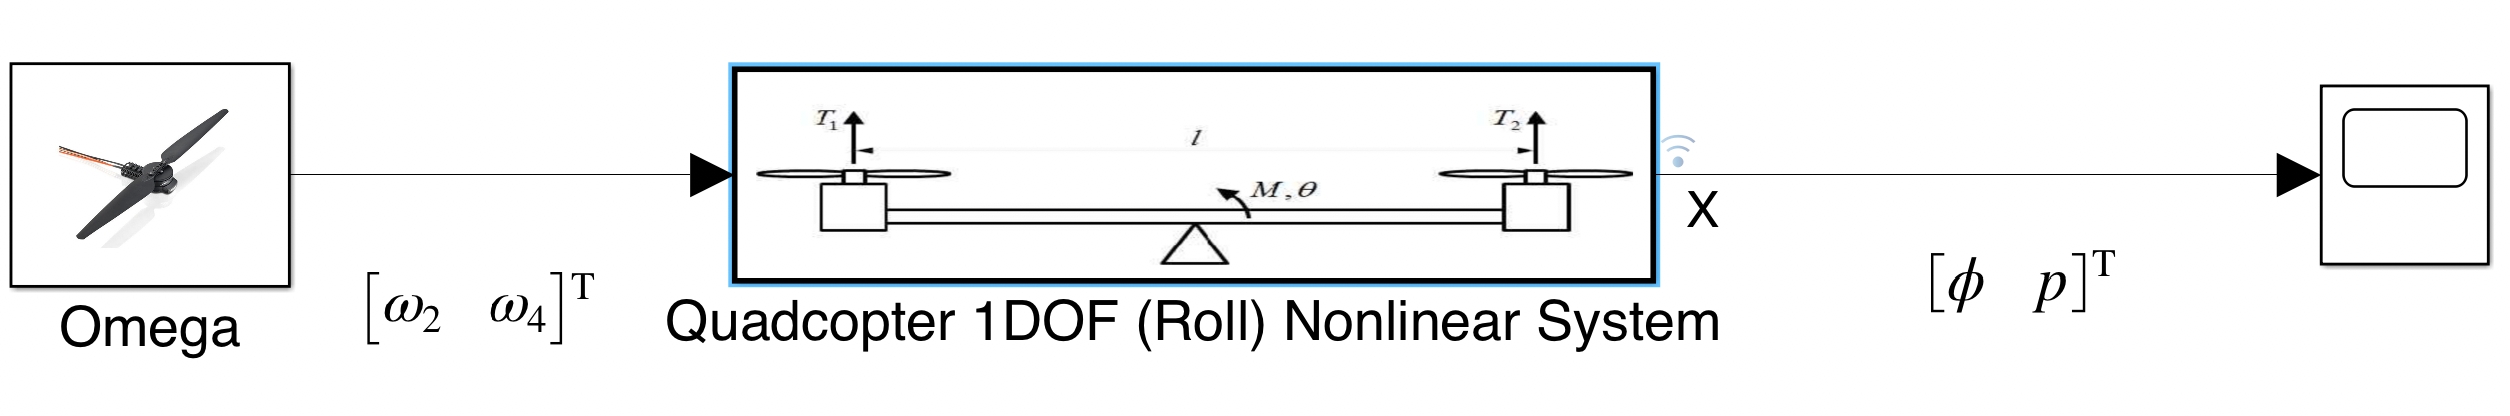
\includegraphics[width=16cm]{../Figures/QuadSimulation/roll_Stand_Model.png}
	\centering
	\vspace*{-15mm}
	\caption{مدل کانال رول استند چهارپره شبیه‌سازی شده در سیمولینک و نمایش ورودی و خروجی‌ها}
	\label{roll_simulink}
\end{figure}

نمایی از داخل بلوک
\lr{Quacopter 1DOF (Roll) Nonlinear System}
در شکل (\ref{Quad1DOF_roll}) آورده شده است.
%\newline
%\newline
\begin{figure}[H]
	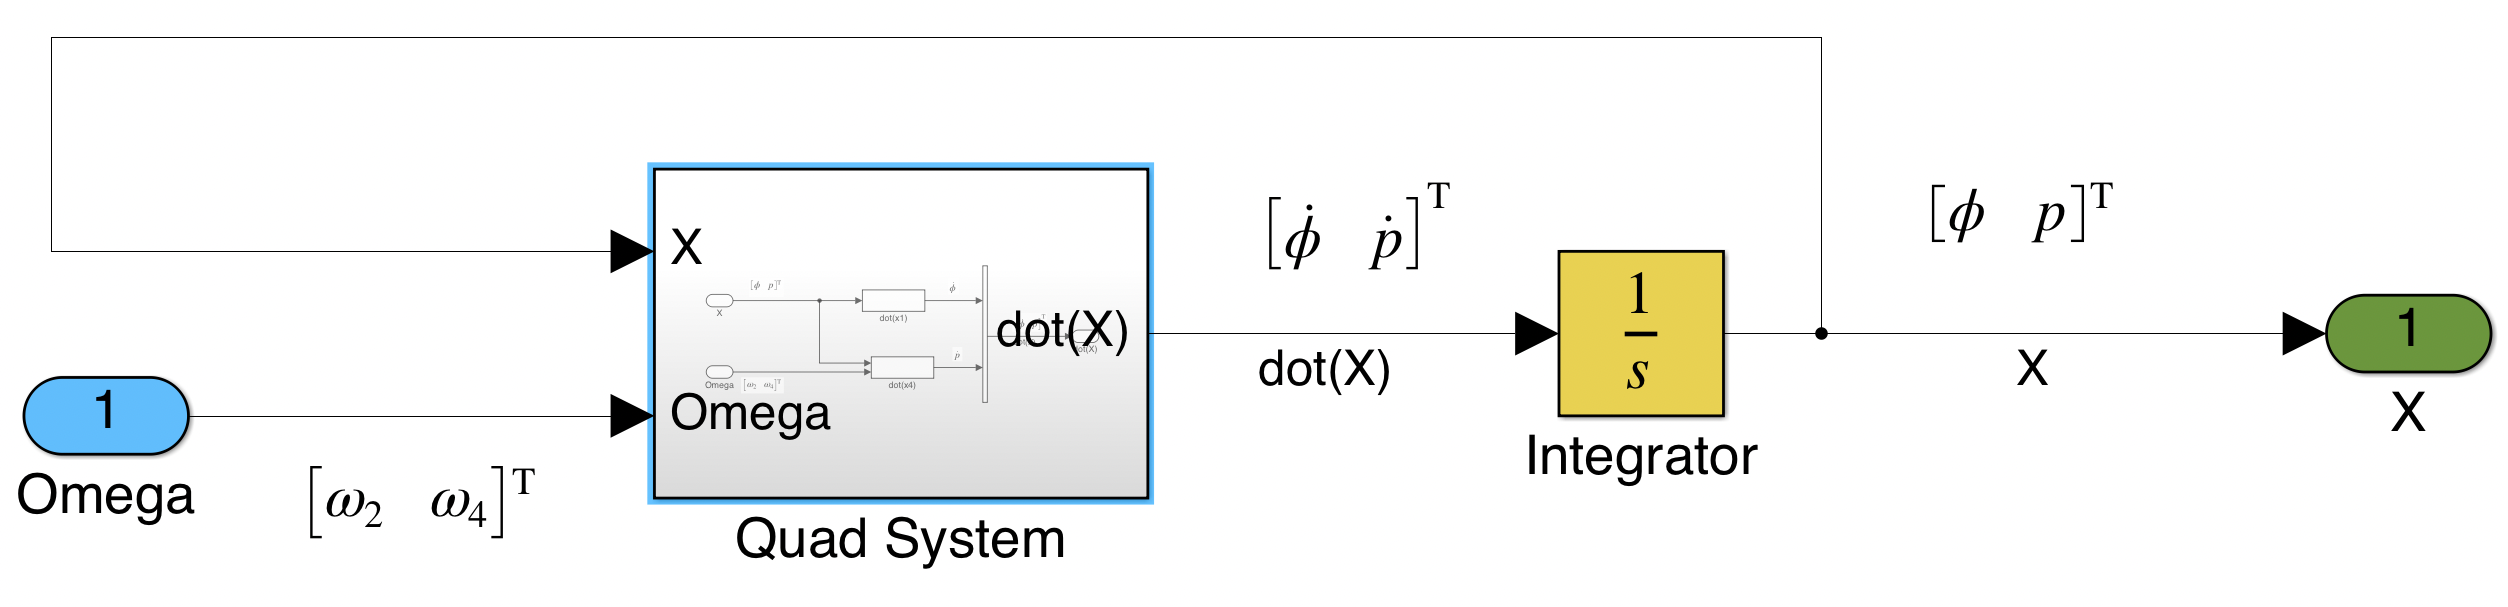
\includegraphics[width=16cm]{../Figures/QuadSimulation/roll_Integrator.png}
	\centering
	\vspace*{-15mm}
	\caption{مدل کانال رول استند چهارپره شبیه‌سازی شده در سیمولینک و نمایش ورودی و خروجی‌ها}
	\label{Quad1DOF_roll}
\end{figure}
بلوک
\lr{Quad System}،
$\dot X$ را به عنوان خروجی می‌دهد. با استفاده از بلوک انتگرالگیر (بلوک زرد رنگ) در شکل
(\ref{Quad3DOF_roll})
از خروجی آن بر اساس شرایط اولیه استند انتگرال گرفته می‌شود و خروجی مورد نیاز ( زاویه رول ($\phi$) و سرعت زاویه‌ای‌
p)
را می دهد.

داخل بلوک
\lr{Quad System}،
دو بلوک دارد که یکی از آن‌های دارای ورودی $X$ و دیگری دارای ورودی $X$ و $\omega$ هستند. مجموع خروحی این دو بلوک $\dot X$ است که برای بلوک
\lr{Quad System}،
نیز اشاره شد.
نمایی از داخل بلوک
\lr{Quad System}
در شکل (\ref{roll_all-six}) آورده شده است.
\begin{figure}[H]
	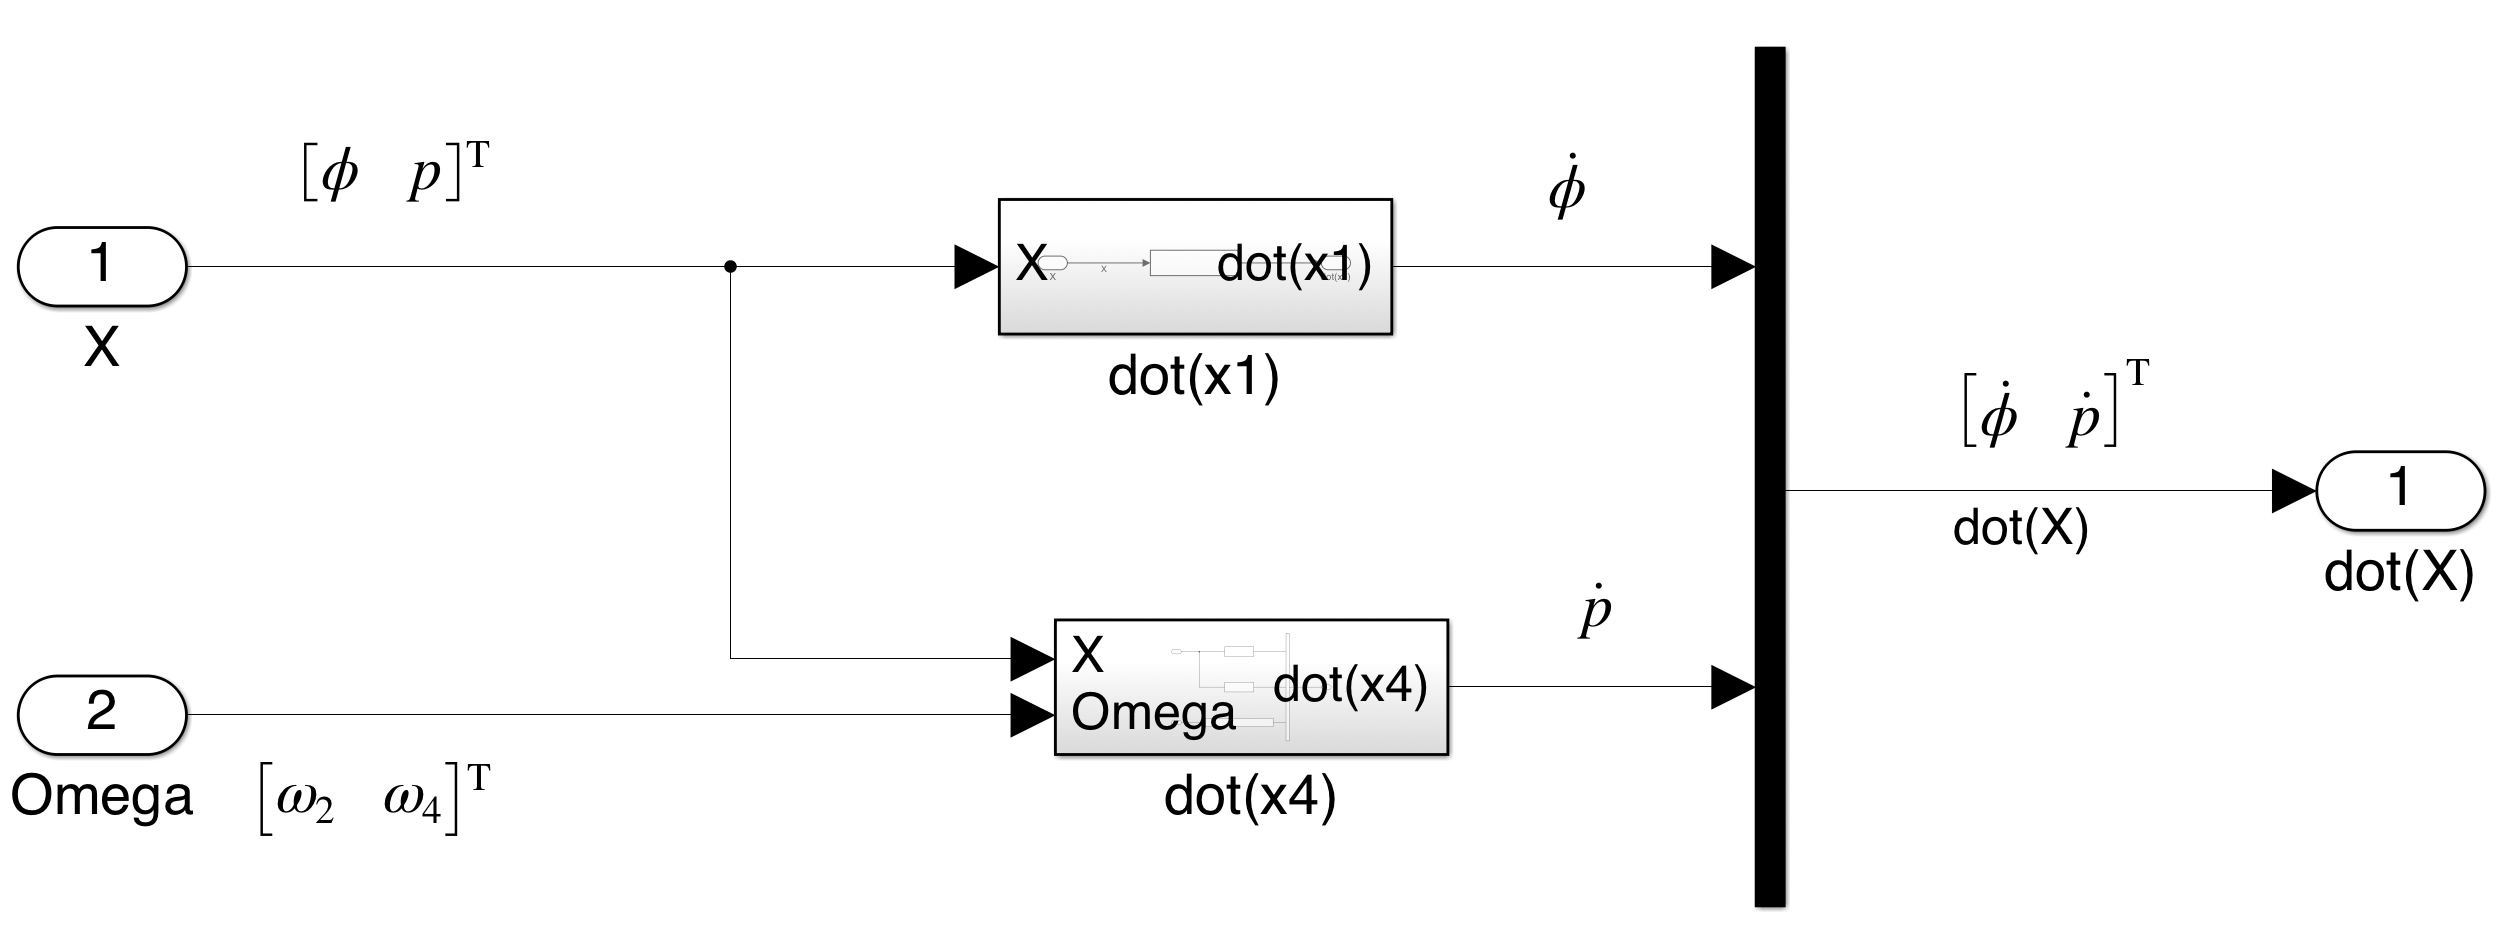
\includegraphics[width=16cm]{../Figures/QuadSimulation/roll_all-six.png}
	\centering
	%	\vspace*{-15mm}
	\caption{نمایی از داخل بلوک \lr{Quad System}}
	\label{roll_all-six}
\end{figure}

\subsection{شبیه سازی کانال پیچ در محیط سیمولینک}
در بخش
(\ref{lin_SISO})
فرم فضای حالت کانال‌های مختلف استند چهار پره بدست آمد در این بخش فرم فضای حالت کانال پیچ در سیمولینک شبیه‌سازی می‌شود.
مدل شبیه‌سازی شده از استند (شکل \ref{pitch_simulink}) دارای دو ورودی سرعت دورانی موتورهای یک و سه  و دارای یک خروجی زاویه‌ی پیچ ($\theta$) و  سرعت زاویه‌ای q است.
\begin{figure}[H]
	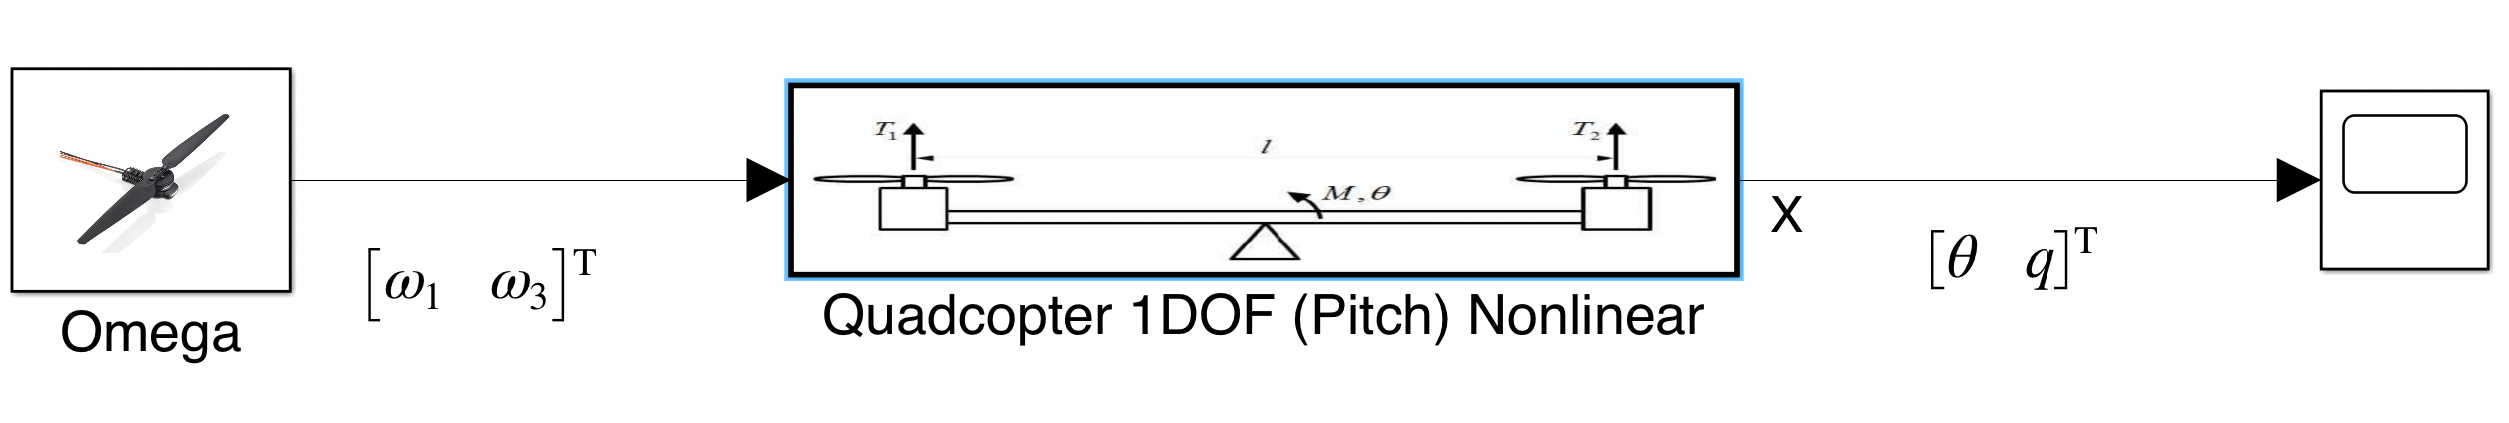
\includegraphics[width=16cm]{../Figures/QuadSimulation/pitch_Stand_Model.png}
	\centering
	\vspace*{-15mm}
	\caption{مدل کانال رول استند چهارپره شبیه‌سازی شده در سیمولینک و نمایش ورودی و خروجی‌ها}
	\label{pitch_simulink}
\end{figure}

نمایی از داخل بلوک
\lr{Quacopter 1DOF (Pitch) Nonlinear System}
در شکل (\ref{Quad1DOF_pitch}) آورده شده است.
%\newline
%\newline
\begin{figure}[H]
	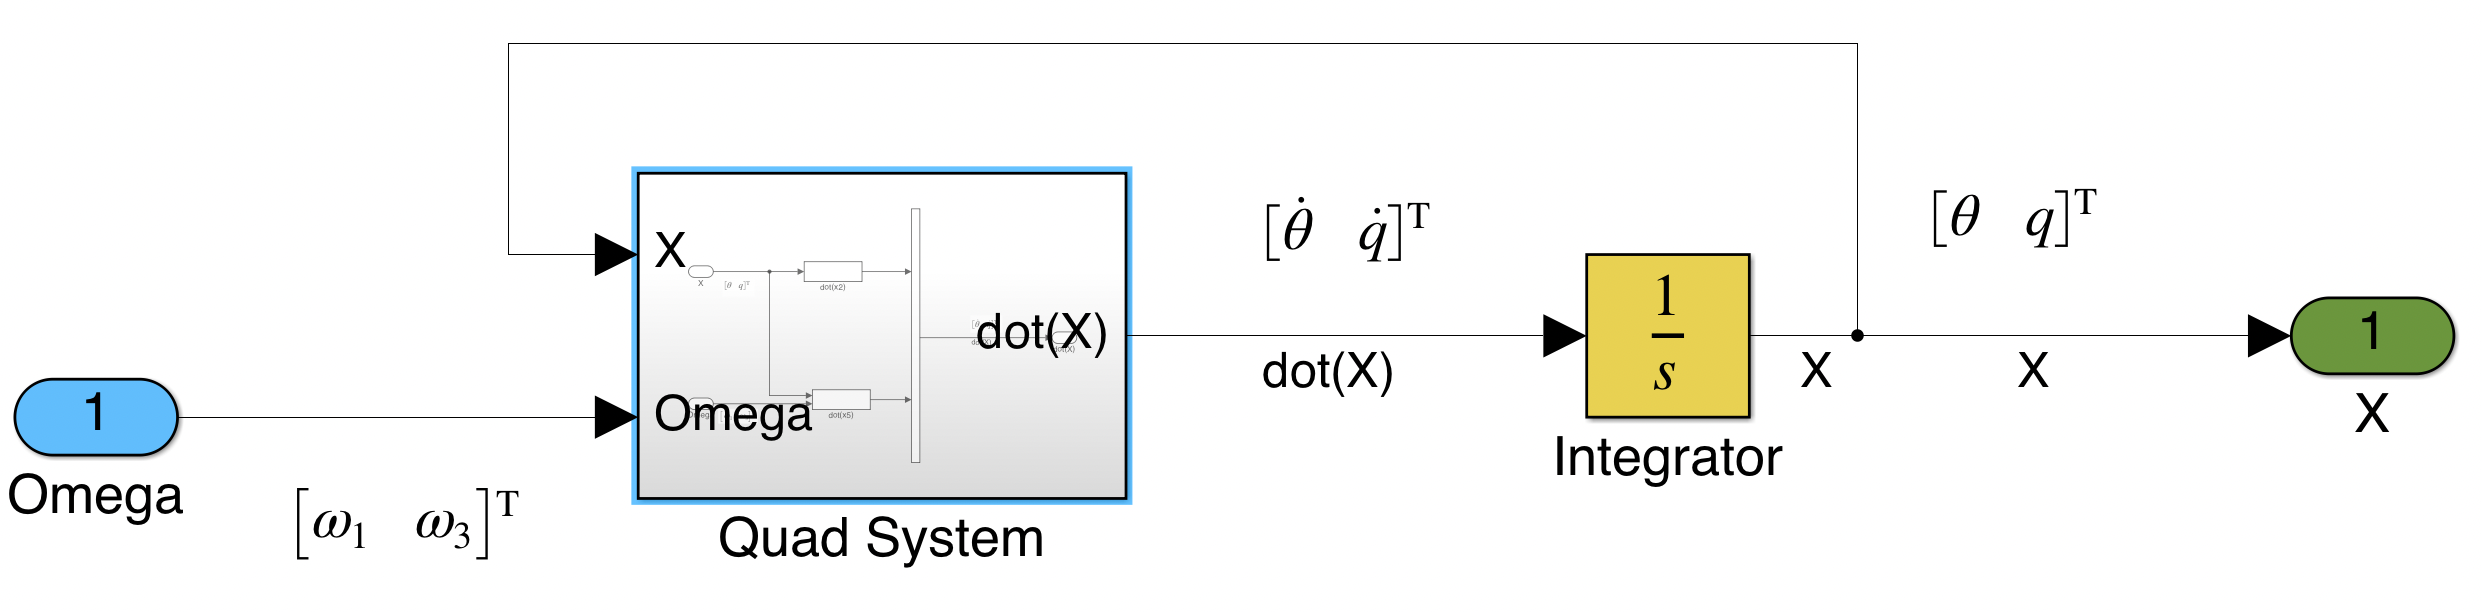
\includegraphics[width=16cm]{../Figures/QuadSimulation/pitch_Integrator.png}
	\centering
	\vspace*{-15mm}
	\caption{مدل کانال رول استند چهارپره شبیه‌سازی شده در سیمولینک و نمایش ورودی و خروجی‌ها}
	\label{Quad1DOF_pitch}
\end{figure}
بلوک
\lr{Quad System}،
$\dot X$ را به عنوان خروجی می‌دهد. با استفاده از بلوک انتگرالگیر (بلوک زرد رنگ) در شکل
(\ref{Quad3DOF_pitch})
از خروجی آن بر اساس شرایط اولیه استند انتگرال گرفته می‌شود و خروجی مورد نیاز ( زاویه پیچ ($\theta$) و سرعت زاویه‌ای‌
q)
را می دهد.

داخل بلوک
\lr{Quad System}،
دو بلوک دارد که یکی از آن‌های دارای ورودی $X$ و دیگری دارای ورودی $X$ و $\omega$ هستند. مجموع خروحی این دو بلوک $\dot X$ است که برای بلوک
\lr{Quad System}،
نیز اشاره شد.
نمایی از داخل بلوک
\lr{Quad System}
در شکل (\ref{pitch_all-six}) آورده شده است.
\begin{figure}[H]
	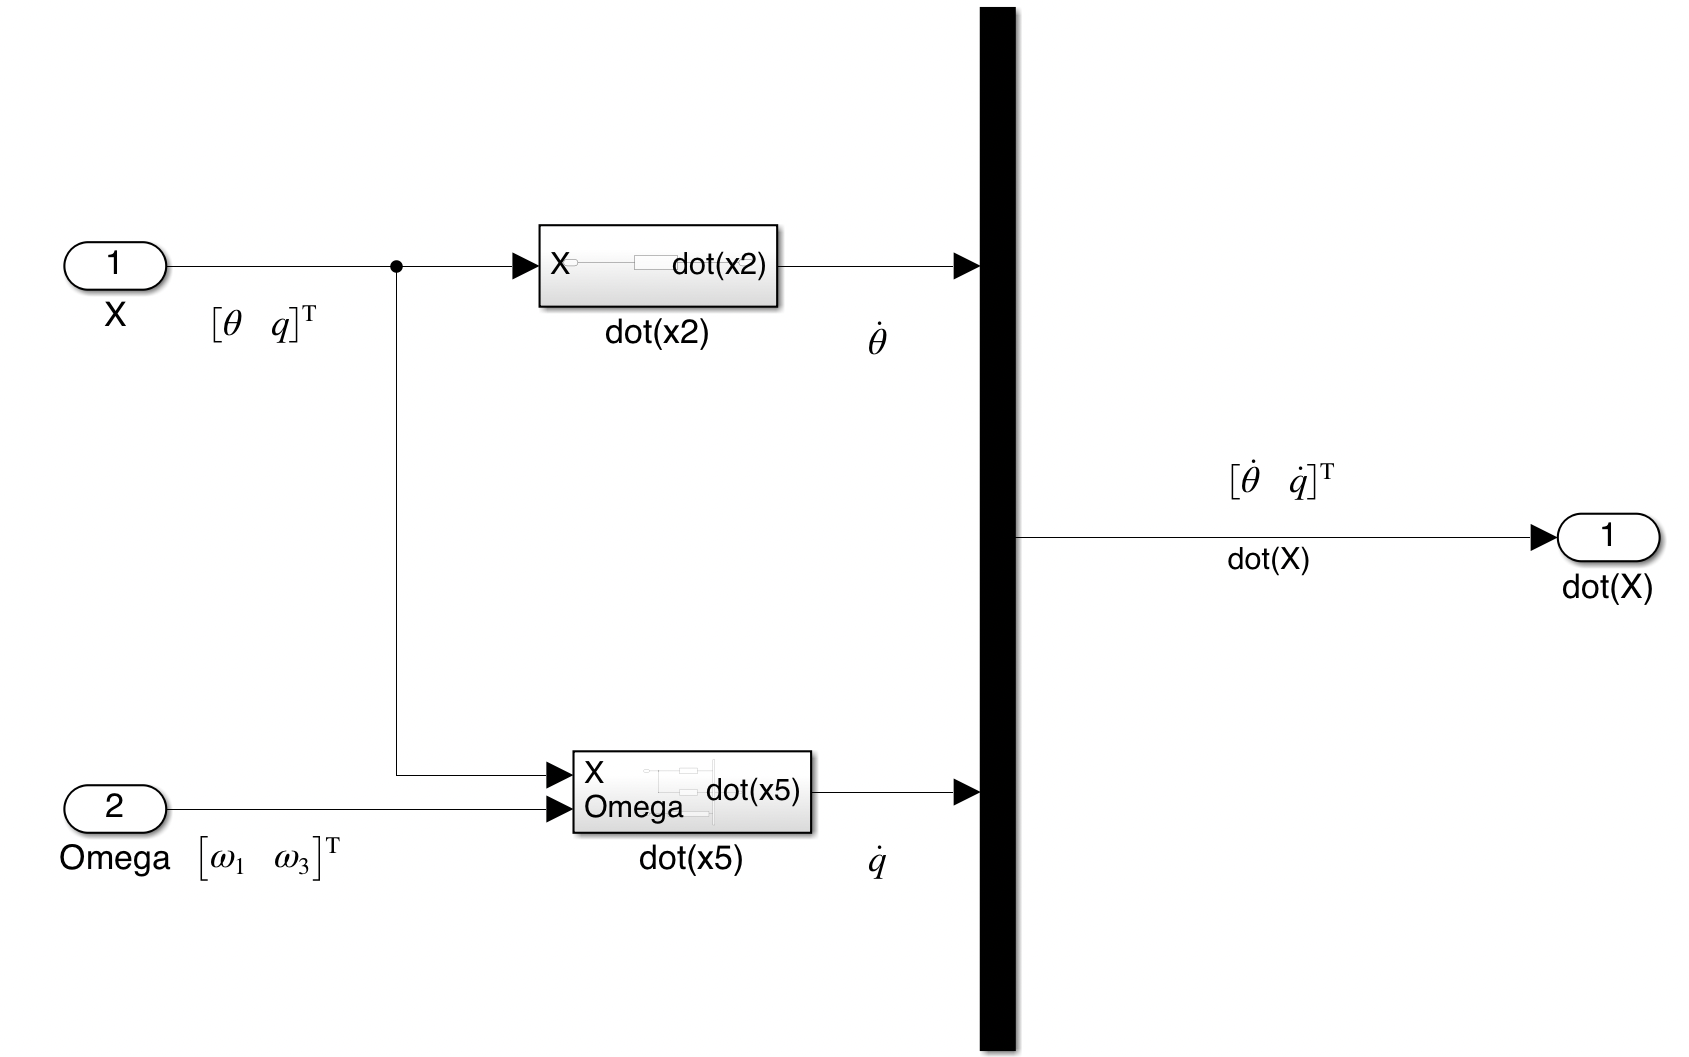
\includegraphics[width=16cm]{../Figures/QuadSimulation/pitch_all-six.png}
	\centering
	%	\vspace*{-15mm}
	\caption{نمایی از داخل بلوک \lr{Quad System}}
	\label{pitch_all-six}
\end{figure}

\subsection{شبیه سازی کانال یاو در محیط سیمولینک}
در بخش
(\ref{lin_SISO})
فرم فضای حالت کانال‌های مختلف استند چهار پره بدست آمد در این بخش فرم فضای حالت کانال رول در سیمولینک شبیه‌سازی می‌شود.
مدل شبیه‌سازی شده از استند (شکل \ref{yaw_simulink}) دارای چهار ورودی سرعت دورانی موتورها  و دارای یک خروجی زاویه‌ی رول ($\psi$) و  سرعت زاویه‌ای r است.
\begin{figure}[H]
	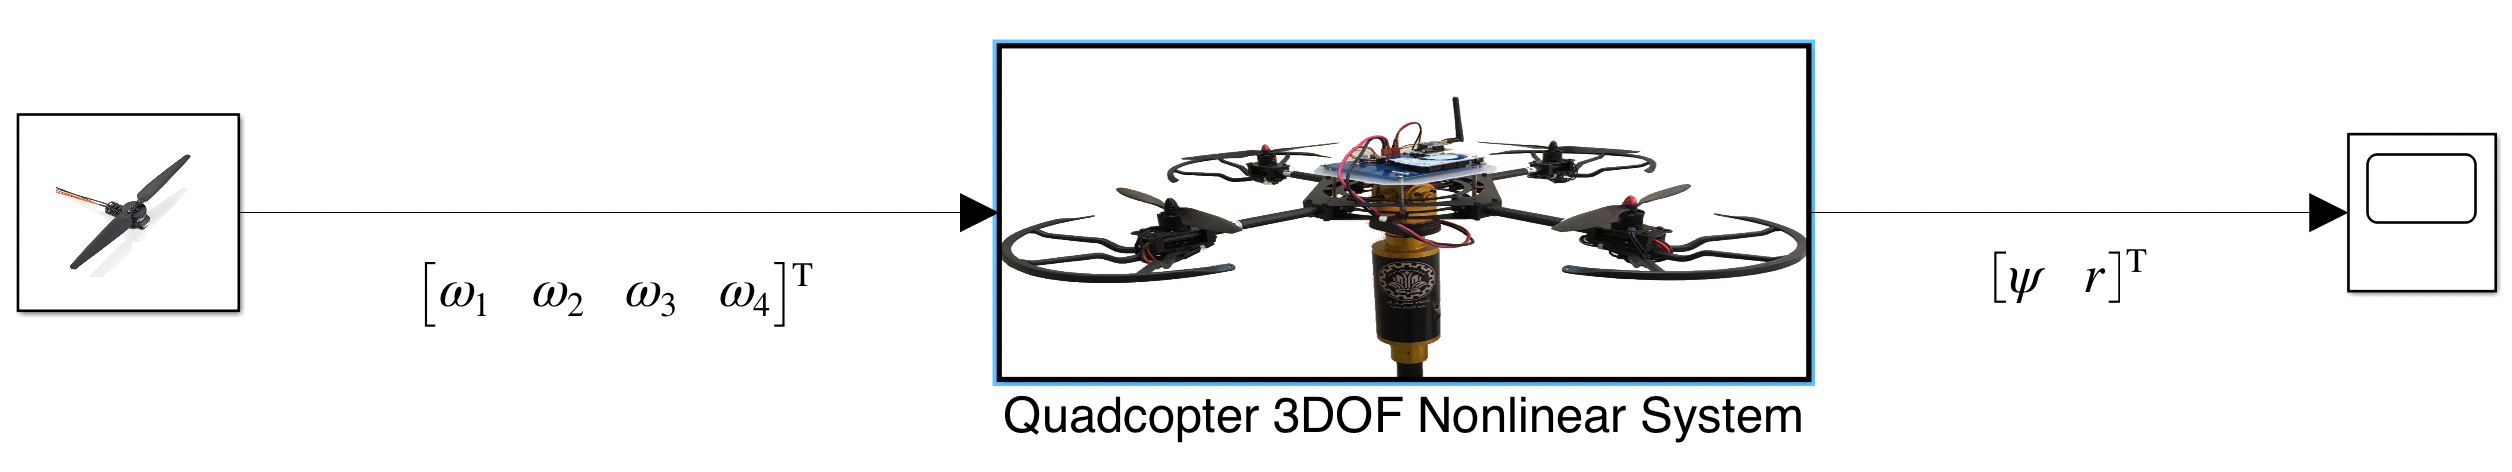
\includegraphics[width=16cm]{../Figures/QuadSimulation/yaw_Stand_Model.png}
	\centering
	\vspace*{-15mm}
	\caption{مدل کانال رول استند چهارپره شبیه‌سازی شده در سیمولینک و نمایش ورودی و خروجی‌ها}
	\label{yaw_simulink}
\end{figure}

نمایی از داخل بلوک
\lr{Quacopter 1DOF (Yaw) Nonlinear System}
در شکل \ref{Quad1DOF_yaw} آورده شده است.
%\newline
%\newline
\begin{figure}[H]
	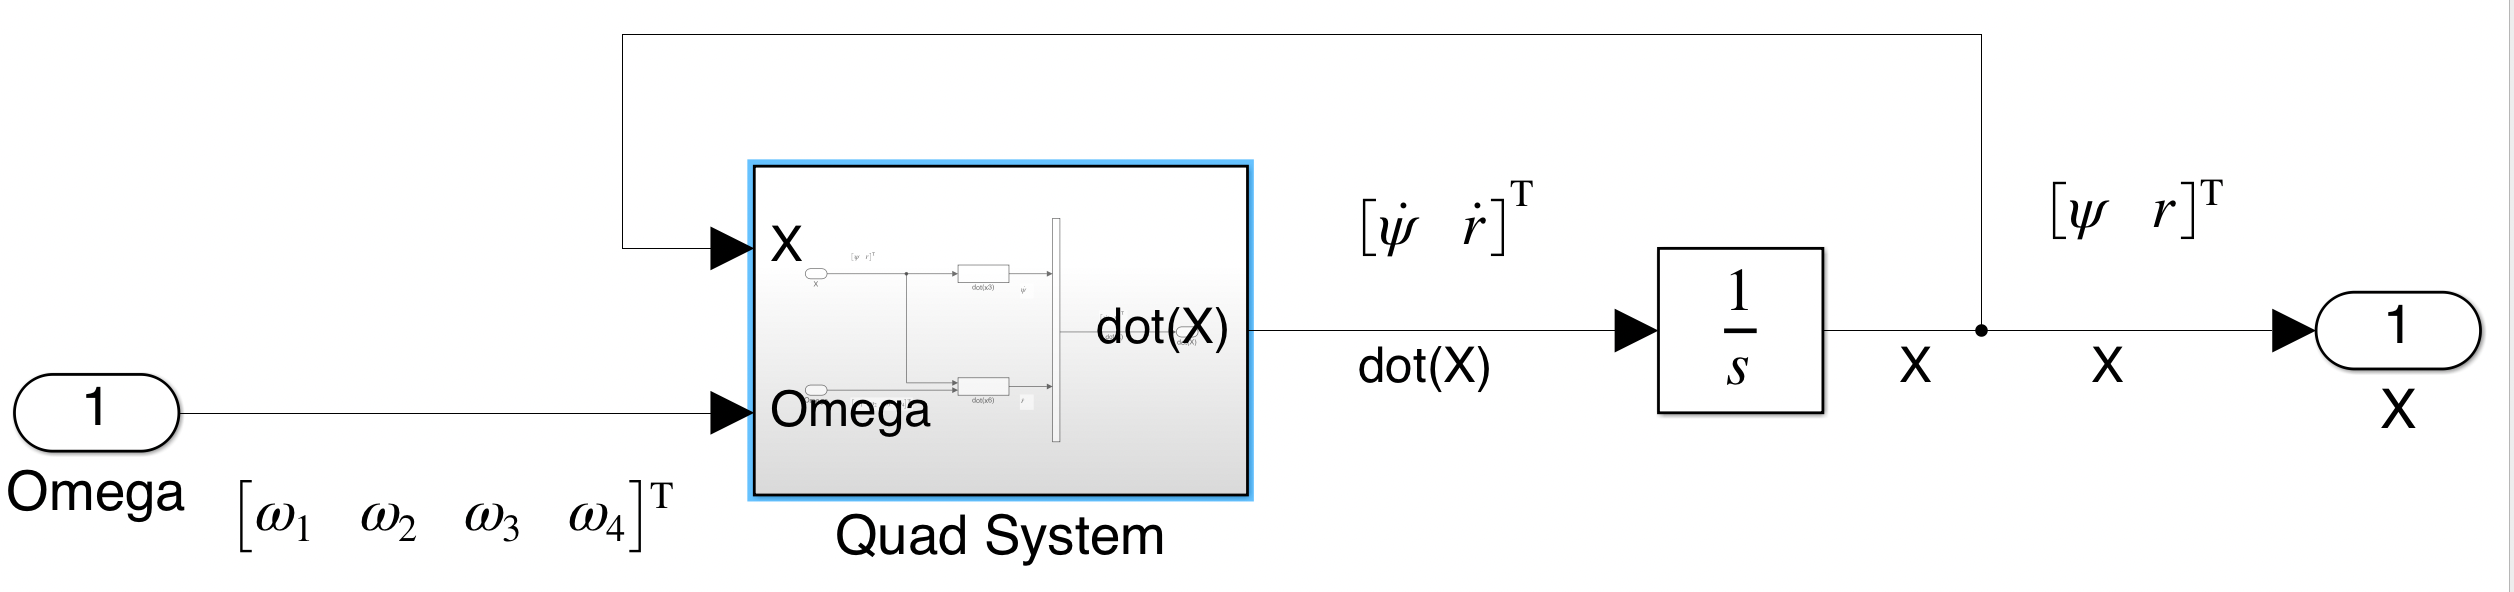
\includegraphics[width=16cm]{../Figures/QuadSimulation/yaw_Integrator.png}
	\centering
	\vspace*{-15mm}
	\caption{مدل کانال یاو استند چهارپره شبیه‌سازی شده در سیمولینک و نمایش ورودی و خروجی‌ها}
	\label{Quad1DOF_yaw}
\end{figure}
بلوک
\lr{Quad System}،
$\dot X$ را به عنوان خروجی می‌دهد. با استفاده از بلوک انتگرال‌گیر (بلوک زرد رنگ) در شکل
\ref{Quad3DOF_pitch}
از خروجی آن بر اساس شرایط اولیه استند انتگرال گرفته می‌شود و خروجی مورد نیاز ( زاویه‌های یاو ($\psi$) و سرعت زاویه‌ای‌
r)
را می دهد.

داخل بلوک
\lr{Quad System}،
دو بلوک دارد که یکی از آن‌های دارای ورودی $X$ و دیگری دارای ورودی $X$ و $\omega$ هستند. مجموع خروحی این دو بلوک $\dot X$ است که برای بلوک
\lr{Quad System}،
نیز اشاره شد.
نمایی از داخل بلوک
\lr{Quad System}
در شکل (\ref{yaw_all-six}) آورده شده است.
\begin{figure}[H]
	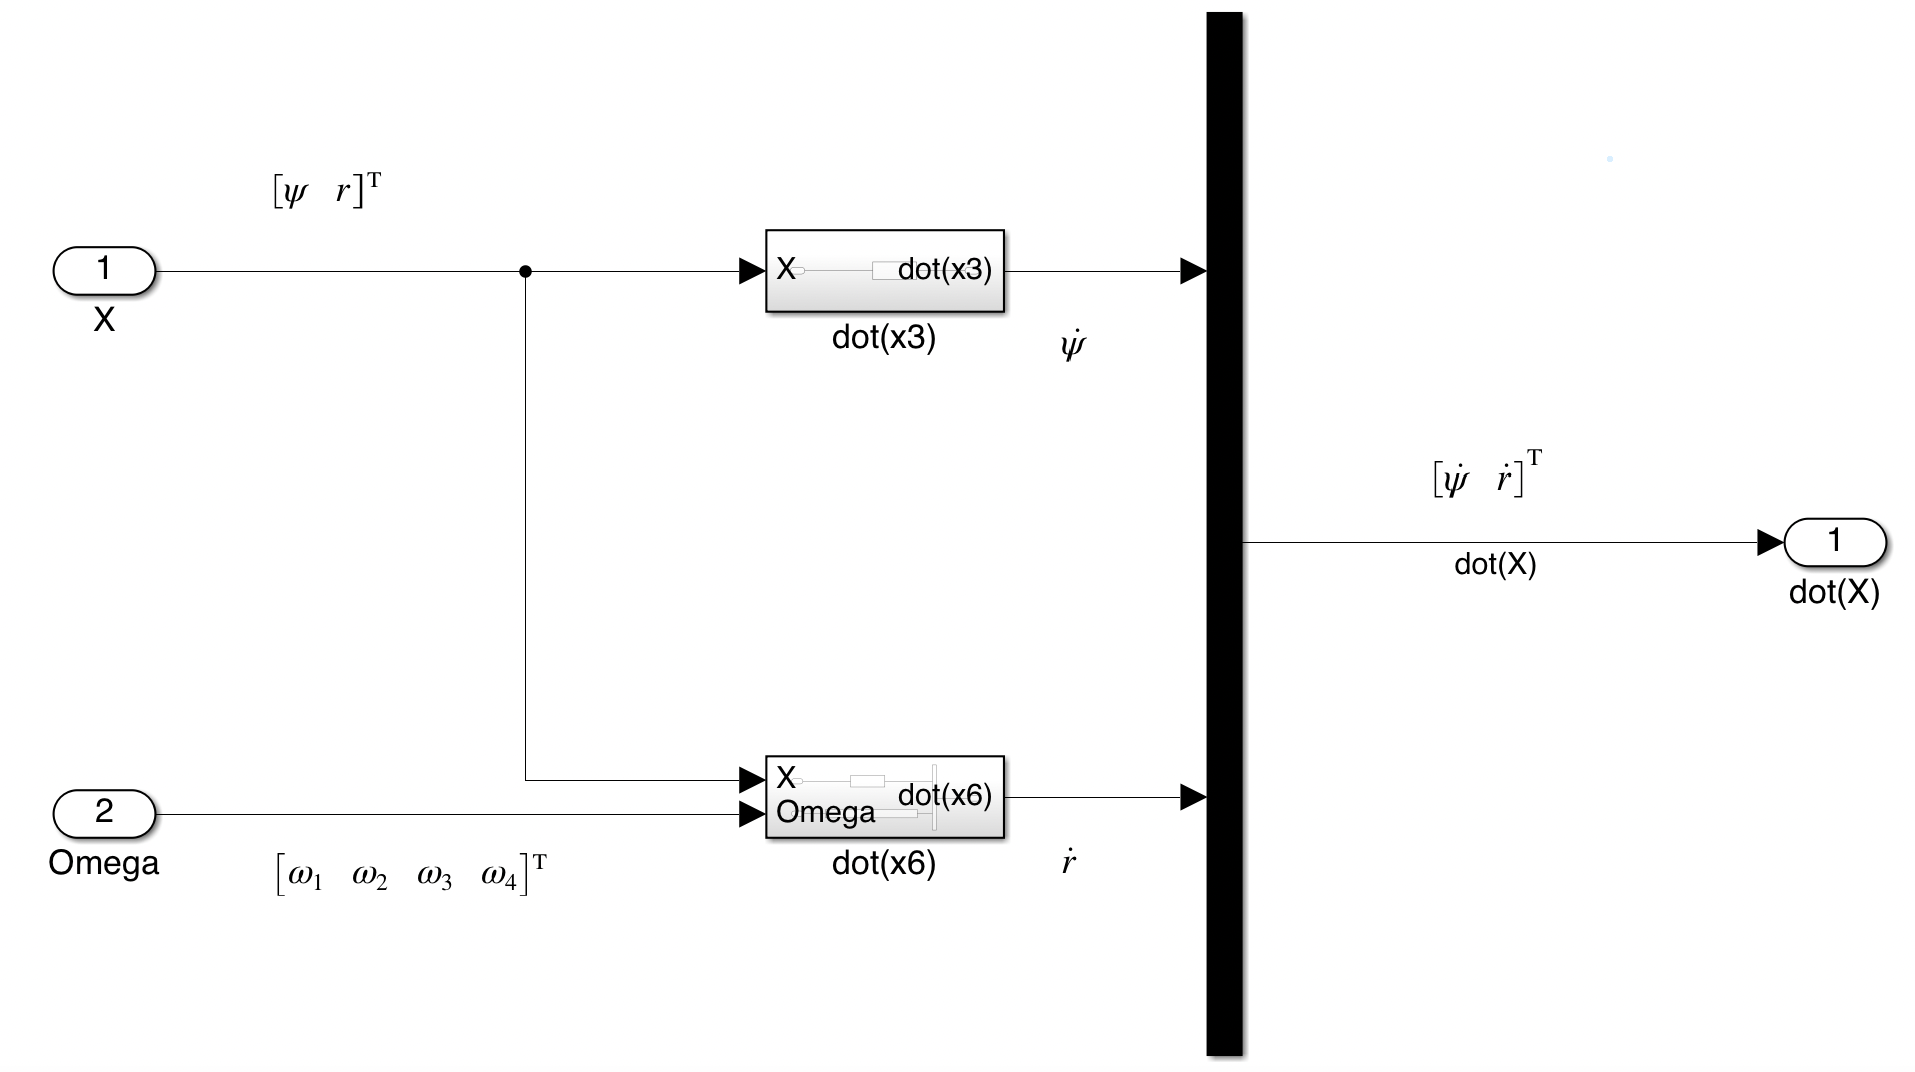
\includegraphics[width=16cm]{../Figures/QuadSimulation/yaw_all-six.png}
	\centering
	%	\vspace*{-15mm}
	\caption{نمایی از داخل بلوک \lr{Quad System}}
	\label{yaw_all-six}
\end{figure}

\subsection{شبیه سازی کانال رول-پیچ در محیط سیمولینک}\label{quadchanell_roll_pitch}
در بخش
\ref{lin_SISO}
فرم فضای حالت کانال‌های مختلف استند چهار پره بدست آمد در این بخش فرم فضای حالت کانال رول در سیمولینک شبیه‌سازی می‌شود.
 فرم فضای حالت استند چهار پره استخراج شد. در شبیه‌سازی نیز از همین روابط استخراج شده استفاده شده است. مدل شبیه‌سازی شده از استند (شکل \ref{roll-pitch_quadsimulink}) دارای چهار ورودی سرعت دورانی موتورها  و دارای دو خروجی زوایای رول ($\phi$) و پیچ ($\theta$)  دو سرعت‌های زاویه‌ای
p
و
q
است.


\begin{figure}[H]
	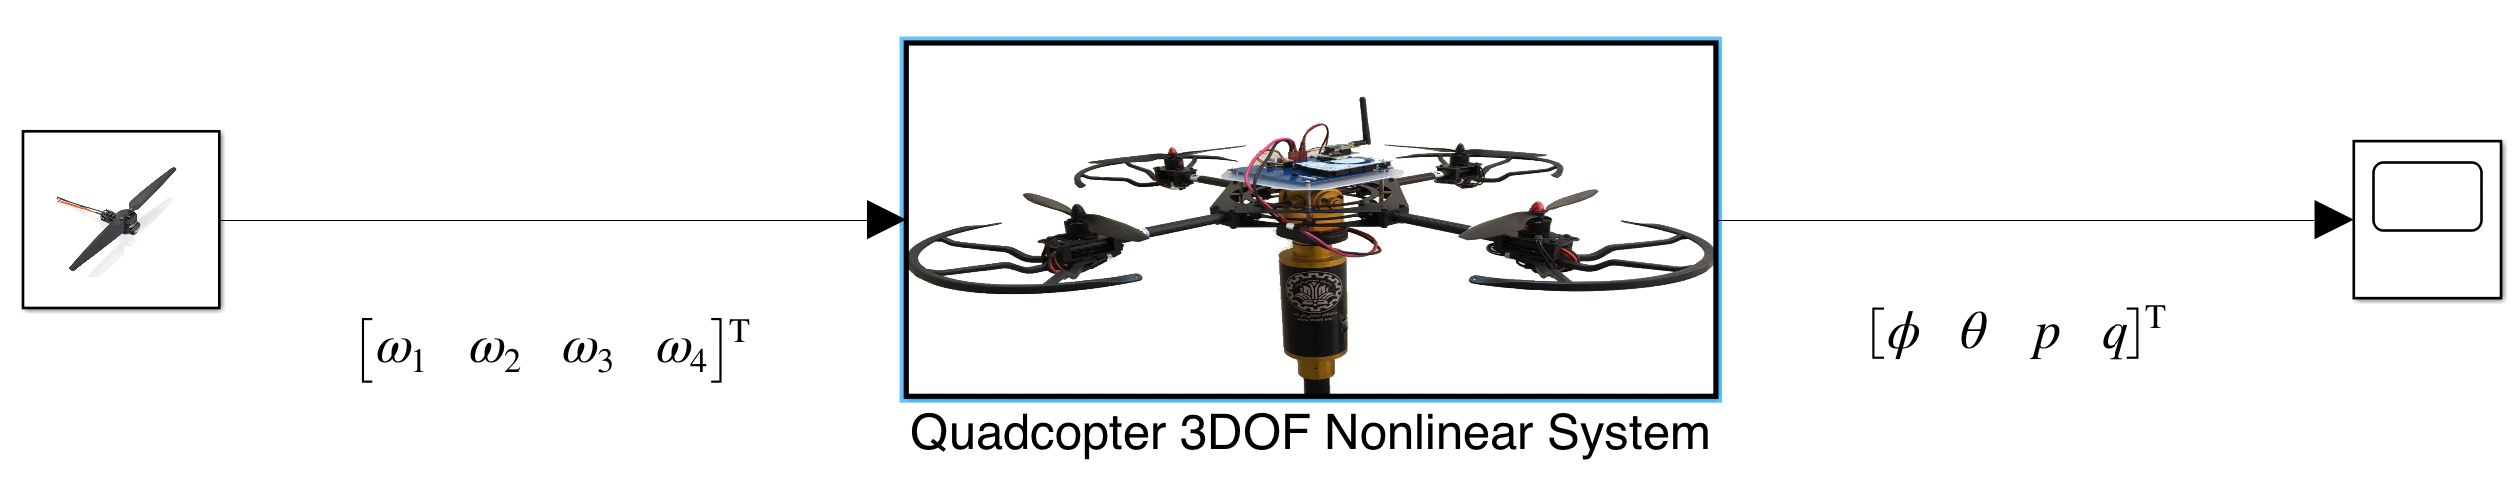
\includegraphics[width=16cm]{../Figures/QuadSimulation/roll-pitch_Stand_Model.png}
	\centering
	\vspace*{-15mm}
	\caption{مدل کانال رول-پیچ استند چهارپره شبیه‌سازی شده در سیمولینک و نمایش ورودی و خروجی‌ها}
	\label{roll-pitch_quadsimulink}
\end{figure}
نمایی از داخل بلوک
\lr{Quacopter 3DOF Nonlinear System}
در شکل (\ref{roll-pitch_Quad3DOF}) آورده شده است.
%\newline
%\newline
\begin{figure}[H]
	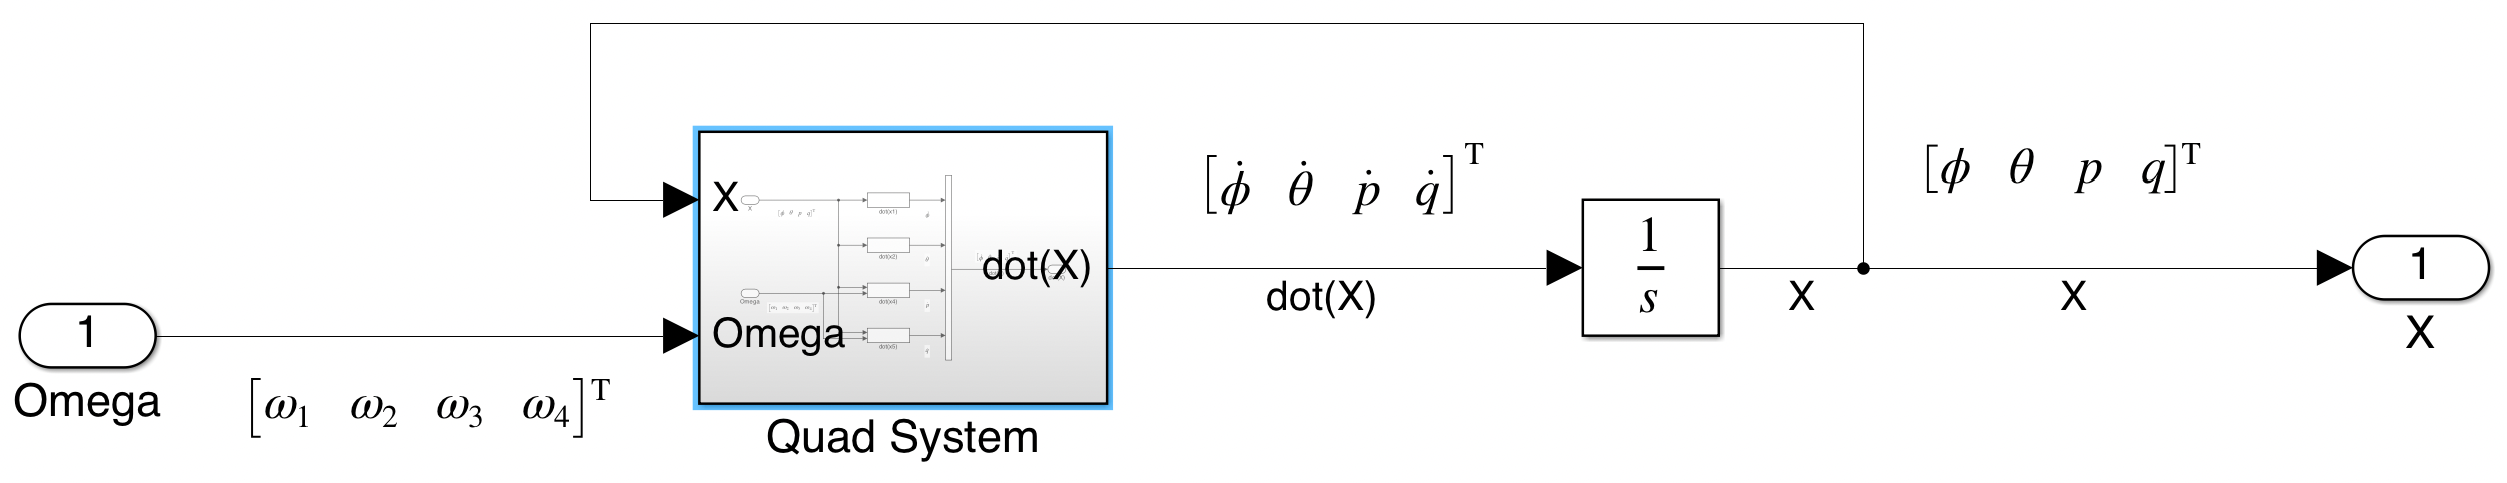
\includegraphics[width=16cm]{../Figures/QuadSimulation/roll-pitch_Integrator.png}
	\centering
	\vspace*{-15mm}
	\caption{مدل کانال رول-پیچ استند چهارپره شبیه‌سازی شده در سیمولینک و نمایش ورودی و خروجی‌ها}
	\label{roll-pitch_Quad3DOF}
\end{figure}
بلوک
\lr{Quad System}،
$\dot X$ را به عنوان خروجی می‌دهد. با استفاده از بلوک انتگرالگیر (بلوک زرد رنگ) در شکل
\ref{roll-pitch_Quad3DOF}
از خروجی آن بر اساس شرایط اولیه استند انتگرال گرفته می‌شود و خروجی مورد نیاز (زاویه‌های رول ($\phi$) و  پیچ ($\theta$) و سرعت‌های زاویه‌ای‌
\lr{p}
و
\lr{q})
را می دهد.

داخل بلوک
\lr{Quad System}،
چهار بلوک دارد که بعضی از آن‌های دارای ورودی $X$ و بعضی از آن‌های دارای ورودی $X$ و $\omega$ هستند. مجموع خروحی این شش بلوک $\dot X$ است که برای بلوک
\lr{Quad System}،
نیز اشاره شد.
نمایی از داخل بلوک
\lr{Quad System}
در شکل \ref{roll-pitch_all-six} آورده شده است.
\begin{figure}[H]
	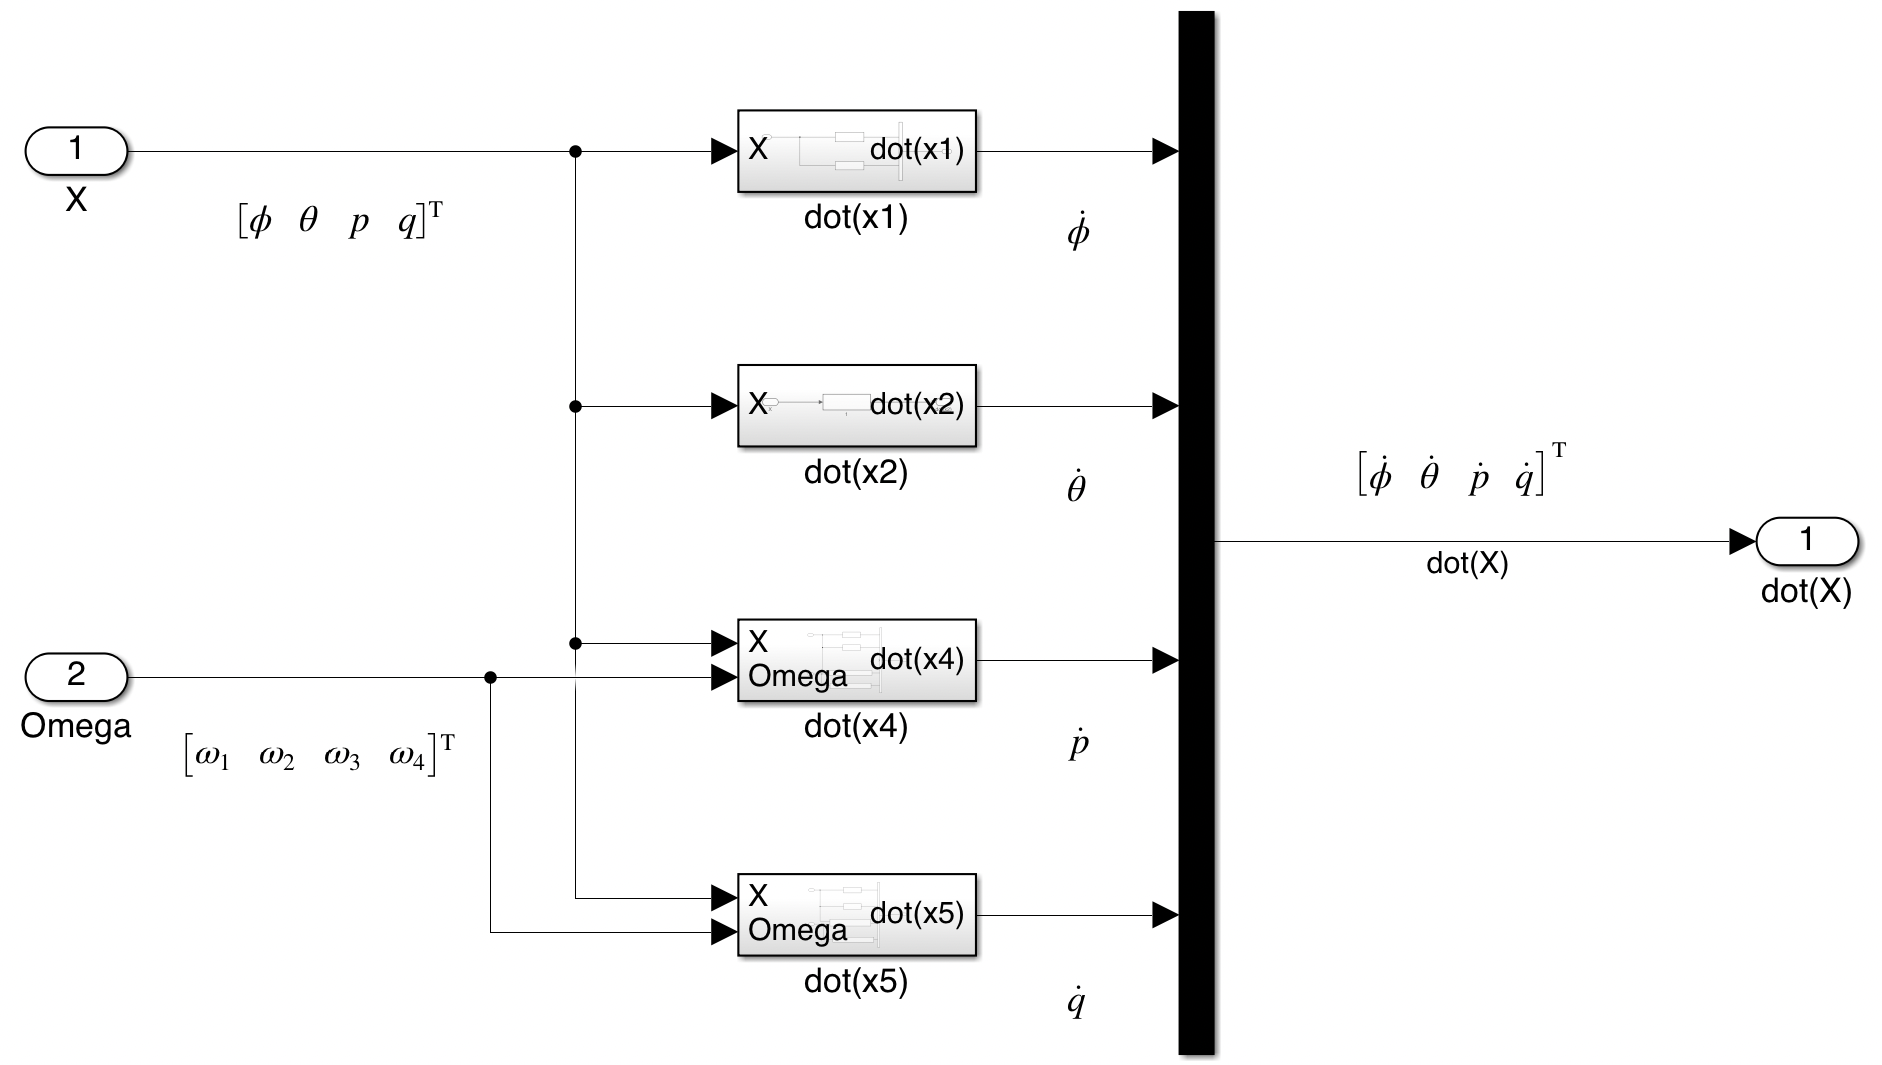
\includegraphics[width=16cm]{../Figures/QuadSimulation/roll-pitch_all-six.png}
	\centering
	%	\vspace*{-15mm}
	\caption{نمایی از داخل بلوک \lr{Quad System}}
	\label{roll-pitch_all-six}
\end{figure}